% COAST -- WACV 2027 Evaluations & Datasets track draft
\documentclass[10pt,twocolumn,letterpaper]{article}
\usepackage[review]{wacv}
\usepackage{graphicx}
\usepackage{amsmath,amssymb}
\usepackage{booktabs,multirow,makecell}
\usepackage{xcolor}
\usepackage[pagebackref,breaklinks,colorlinks]{hyperref}

\def\paperID{****}
\def\confName{WACV}
\def\confYear{2027}
\newcommand{\coast}{\textsc{COAST}}
\newcommand{\method}[1]{\textsc{#1}}
\newcommand{\pending}[1]{\textcolor{red}{[#1]}}

\begin{document}
\title{COAST: A Cross-Organ Benchmark and Conditioning Study for\\
Histology-to-Transcriptomics Prediction}
\author{Anonymous WACV submission\\Paper ID \paperID}
\maketitle

\begin{abstract}
Models that predict spatial gene expression from H\&E images are usually tested on new patients from
an organ seen during training. This does not tell us whether they work on a new organ. We present
\coast{}, a controlled benchmark for this harder setting. \coast{} separates prediction for new
patients from known organs from transfer to a completely unseen organ. It uses patient-disjoint
splits, selects genes from training data only, and gives every method the same frozen image features,
gene panels, and metrics. Across HEST-1k and STImage-1K4M, all model families perform substantially
worse when the test organ is unseen. We also find that Pearson correlation can become uninformative:
some training-selected genes are almost silent in the test organ, leaving too little target variation
to measure correlation reliably. Finally, we add the same inference-available morphology conditioner
to six representative regression and spatial architectures, including a recent Gene-DML-style
multi-level predictor. It improves all six in both evaluation
settings, with the largest gains for models that do not already combine local and slide-level context.
The gain persists on the recent model and is largest under organ shift. Additional architecture
screening, including neutral and negative cases, is reported in the appendix.
Thus, FiLM is useful across several prediction families, but its benefit depends on the information
already present in a model. \coast{} turns cross-organ generalization from
an implicit claim into a reproducible test. We will release the splits, panels, predictions, and code.
\end{abstract}

\begin{figure*}[t]
\centering
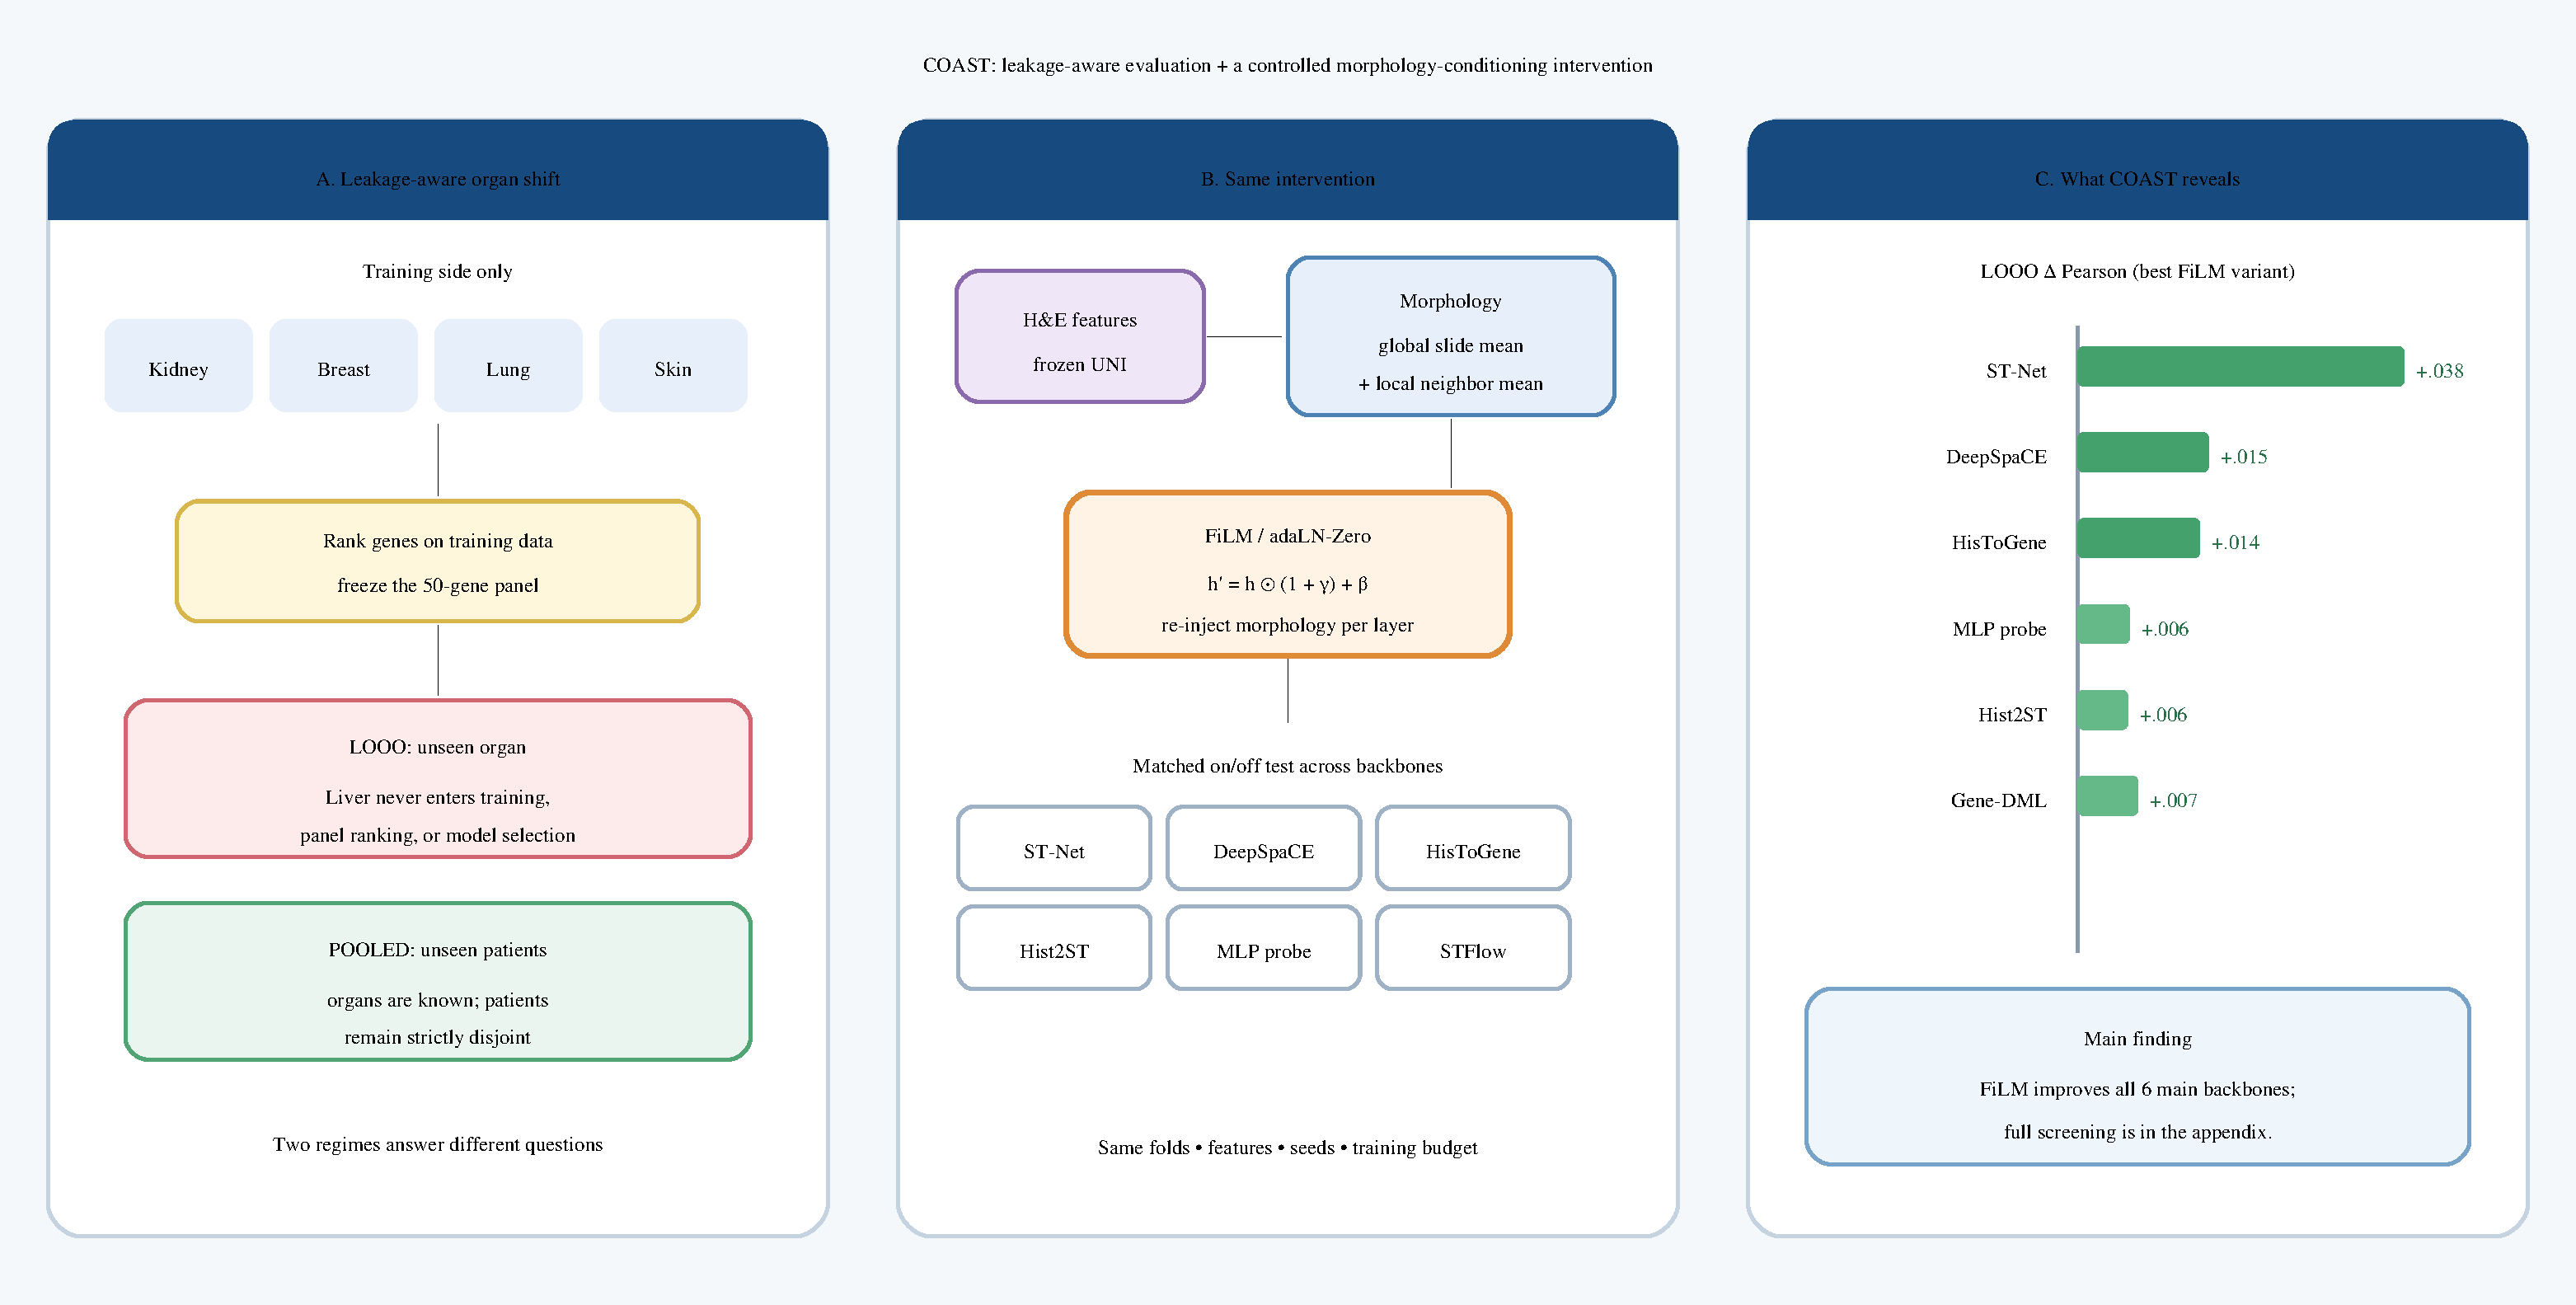
\includegraphics[width=\textwidth]{figures/coast_overview.pdf}
\caption{\textbf{The COAST contribution.} (A) Patient-disjoint POOLED and organ-held-out LOOO
evaluation use gene panels ranked only on training data. (B) The same inference-available global/local
morphology intervention is tested against each backbone's unconditioned version. (C) It improves all
six representative backbones shown in the main study. The appendix reports the complete screening,
including neutral and negative cases.}
\label{fig:overview}
\end{figure*}
\section{Introduction: the missing test}
\label{sec:intro}
Spatial transcriptomics (ST) shows where genes are expressed inside tissue~\cite{spatialtx,xenium}.
It is informative but expensive. H\&E slides are routine and much cheaper, so many methods now try to
predict spatial expression directly from histology. They use regression, transformers, spatial graphs,
retrieval, multi-resolution features, or generative models
~\cite{stnet,histogene,hist2st,bleep,triplex,stflow}.

The usual test holds out a patient but keeps the organ the same. A breast test slide, for example, is
predicted by a model that has already seen other breast slides. This measures performance on a new
patient, but not on new tissue. Our question is simple: \emph{what happens when the test organ was never
seen during training?} This matters because paired ST data are scarce and uneven across organs.

This test is easy to get wrong. If genes are selected using all slides, the test organ influences what
is evaluated. If genes are correctly selected from training slides only, some may be almost silent in
the new organ. Pearson correlation then has little variation to measure. A low score can reflect model
error, a mismatched gene panel, or both. Reporting only one average hides this distinction.

We introduce \coast{} (\textbf{C}ross-\textbf{O}rgan \textbf{A}ssessment of \textbf{S}patial
\textbf{T}ranscriptomics prediction). It separates new-patient prediction (POOLED) from new-organ
transfer (LOOO), selects genes from training data only, and reports detectability and target variance
beside accuracy. We apply it to HEST-1k~\cite{hest} and STImage-1K4M~\cite{stimage}. Every method uses
the same frozen UNI image features~\cite{uni}, allowing us to compare predictors rather than encoders.
Figure~\ref{fig:overview} summarizes the split, the shared intervention, and the main result.

We ask four questions:
\begin{enumerate}
  \item How much performance is lost when the test organ is unseen?
  \item Do model rankings change between new-patient and new-organ evaluation?
  \item When does Pearson correlation stop separating models reliably?
  \item Does the same morphology conditioner help different architectures?
\end{enumerate}

The fourth question makes the benchmark diagnostic, not only descriptive. In the main conditioning
study, FiLM improves six representative regression and spatial backbones in both regimes, including
a recent multi-level Gene-DML-style predictor. The
appendix reports the complete architecture screening, including cases where the intervention is neutral
or harmful. This gives a clear result: morphology conditioning often helps, but its value depends on
the prediction architecture.

Our contributions are:
\begin{itemize}
  \item \textbf{A clean cross-organ test:} patient-disjoint POOLED and LOOO splits, genes ranked on
  training data only, equal weighting of organs, and released evaluation artifacts.
  \item \textbf{A metric diagnosis:} low gene detection and target variance identify cases where
  Pearson correlation cannot meaningfully separate models.
  \item \textbf{A controlled intervention:} the same morphology conditioner improves six
  representative architectures in both regimes; complete screening is reported in the appendix.
\end{itemize}

\section{Related Work}
\label{sec:related}
\paragraph{Histology-to-expression prediction.}
ST-Net~\cite{stnet} predicts each spot with a CNN; HisToGene~\cite{histogene} and
Hist2ST~\cite{hist2st} introduces spatial graphs, while STFlow~\cite{stflow} models the joint
expression field with whole-slide flow matching. Contrastive retrieval and multi-resolution
aggregation provide further comparison families~\cite{bleep,triplex}, reported in the appendix.
These advances primarily optimize within-cohort accuracy. \coast{} is complementary: it holds image
features, panels, partitions, and metrics fixed to examine conclusions under organ shift. Recent
vision methods add multi-level discrimination (Gene-DML~\cite{genedml}) and fully connected,
negative-aware spatial attention (FEAST~\cite{feast}). These context-rich designs are important tests
for COAST because they may change both cross-organ rankings and the value of extra conditioning.

\paragraph{Pathology representations and ST resources.}
Foundation encoders transfer morphology across cohorts; examples include UNI~\cite{uni},
Prov-GigaPath~\cite{gigapath}, CONCH~\cite{conch}, and Virchow~\cite{virchow}. We use frozen UNI
features for every method rather than confounding evaluation with encoder choice. HEST-1k~\cite{hest}
and STImage-1K4M~\cite{stimage} provide paired slides and expression across organs. We reorganize
these resources around organ-held-out assessment rather than proposing a new biological dataset.

\paragraph{Benchmarks for multimodal pathology.}
Recent benchmarks study image--gene representation learning across organs, encoders, and downstream
tasks~\cite{hescape}. COAST addresses a distinct evaluation gap in supervised expression prediction:
the test organ is absent from training, target genes are selected without test expression, and model
accuracy is interpreted together with target detectability. It further uses a shared conditioning
intervention to compare how prediction architectures respond under the same shift.

\paragraph{Evaluation under distribution shift.}
Biomedical benchmarks can overstate generalization when patient, site, acquisition, label-selection,
or preprocessing information crosses split boundaries. In histology-to-ST prediction, organ shift
also changes the marginal distribution and detectability of the targets themselves. Our focus is
therefore not only a stricter split, but an audit of how target shift interacts with the dominant
correlation metric and with scientific conclusions.

\section{COAST: a controlled cross-organ test}
\label{sec:protocol}
COAST follows three rules: the test organ cannot affect training or target selection; new patients
and new organs must be reported separately; and accuracy must be accompanied by information about
whether the target genes are measurable. These rules turn two public datasets into a reproducible
stress test.

Let a slide contain patch features $\mathbf Z\in\mathbb R^{N\times d}$, spot coordinates
$\mathbf C\in\mathbb R^{N\times2}$, and expression $\mathbf Y\in\mathbb R^{N\times g}$. A model
trained on organs $\mathcal O_{\rm tr}$ is evaluated on slides from either known organs or an organ
$o\notin\mathcal O_{\rm tr}$. All slides from a patient remain in one partition.

\subsection{Separate new patients from new organs}
\paragraph{LOOO: unseen-organ transfer.}
For each organ $o$, all cohorts and patients of $o$ are excluded from training and used only for the
final test. Model selection uses a fixed validation partition drawn from the remaining organs; the
test organ is not used for early stopping, hyperparameter selection, or threshold selection.

\paragraph{POOLED: known-organ deployment.}
All organs occur in training, but complete patients are held out within each organ. This evaluates a
single multi-organ model on new patients without conflating that question with unseen-organ transfer.

\begin{table}[t]
\centering\small
\setlength{\tabcolsep}{3.6pt}
\resizebox{\columnwidth}{!}{%
\begin{tabular}{lccc}
\toprule
Protocol & Patient held out & Organ held out & Primary question\\
\midrule
Within cohort & yes & no & in-distribution\\
\coast{}-POOLED & yes & no & multi-organ deployment\\
\coast{}-LOOO & yes & yes & organ transfer\\
\bottomrule
\end{tabular}
}
\caption{The protocols answer different questions and must be reported separately.}
\label{tab:regimes}
\end{table}

\subsection{Choose genes without looking at the test organ}
For fold $f$, we first form the technically compatible gene universe $A_f$ using assay annotations,
without inspecting held-out expression. We then rank genes by pooled log-transformed variance on
training slides only:
\begin{equation}
G_f=\operatorname{TopK}_{g\in A_f}
\operatorname{Var}_{(s,i)\in D^{f}_{\rm tr}}
\!\left[\log(1+Y_{sig})\right],\qquad K=50.
\label{eq:panel}
\end{equation}
The selected $G_f$ is frozen before validation and test evaluation. We release both $A_f$ and $G_f$
so that technical availability cannot be confused with expression-based selection. Clinically defined
genes are reported as a separate, predeclared analysis rather than inserted after inspecting results.

\subsection{Report when the target is measurable}
The primary endpoint is macro-averaged gene-wise Pearson correlation: calculate correlation over
spots for each nonconstant gene on each slide, average within slide, then give each organ equal weight.
We additionally report Spearman correlation, normalized RMSE, MAE, and detection average precision.
Micro (slide-weighted) means are secondary because HEST contains 2--24 slides per organ.

For every organ we report the fraction of spots with nonzero expression, median target variance, and
the number of evaluable genes. These are diagnostics, not inputs to the model. A detection-aware PCC
restricted to genes satisfying a threshold $\tau$ is a predeclared secondary endpoint; $\tau$ is fixed
without optimizing test performance and sensitivity is shown over several thresholds. Uncertainty is
estimated by a patient/slide bootstrap nested within organ and by three training seeds.

\subsection{Two complementary datasets}
HEST comprises 72 slides grouped into eight organs and spans Visium and Xenium; the distribution is
highly imbalanced. STImage-1K4M contributes 80 Visium slides, ten for each of eight organs, but its
released slides are heavily downsampled. Table~\ref{tab:data} reports the evaluation units.

\begin{table}[t]
\centering\small
\setlength{\tabcolsep}{3.5pt}
\resizebox{\columnwidth}{!}{%
\begin{tabular}{lrrr}
\toprule
Dataset / organ & Slides & Mean spots & Platform\\
\midrule
\multicolumn{4}{l}{\emph{HEST (72 slides)}}\\
Breast / Kidney / Colorectal / Prostate & 8/24/8/23 & 6938/3092/3007/2727 & mixed/Vis./Vis./Vis.\\
Lung / Pancreas / Liver / Skin & 2/3/2/2 & 2603/2524/2098/1517 & Xen./Xen./Vis./Xen.\\
\midrule
\multicolumn{4}{l}{\emph{STImage-1K4M (80 slides)}}\\
8 organs & 10 each & 942--3605 & Visium\\
\bottomrule
\end{tabular}
}
\caption{Cross-organ evaluation resources. Exact patient-level partitions are released as machine-readable files.}
\label{tab:data}
\end{table}

\subsection{Make every result traceable}
Each reported cell is tied to a versioned split file, panel file, prediction file, and evaluation
configuration. Code records patient identifiers after de-identification, training/validation/test
membership, seed, checkpoint selected on validation only, preprocessing version, and metric policy.
No test prediction is used to select a checkpoint or reporting threshold.

\section{Models and the shared FiLM intervention}
\label{sec:models}
The paper contains two linked studies. The \emph{benchmark study} compares representative predictors
under identical COAST inputs. The \emph{conditioning study} changes one factor inside each predictor:
whether global or local morphology is injected through FiLM. Keeping these studies separate prevents
a strong backbone from being mistaken for evidence that conditioning itself works.

\subsection{Give every method the same inputs}
Every method receives identical frozen 1024-dimensional UNI patch features, coordinates, fold-specific
panels, and normalized targets. The main paper evaluates linear ridge and random-forest probes;
ST-Net, DeepSpaCE, an MLP probe, HisToGene, Hist2ST, a Gene-DML-style multi-level predictor,
and the whole-slide STFlow generator. This covers
spot-independent regression, slide transformers, graph/spatial models, and generative prediction.
The appendix contains the complete screening table, including retrieval and multi-resolution models.
Training budgets and validation rules are matched where model
interfaces permit; all deviations are disclosed rather than silently harmonized.

\subsection{Change one factor: morphology conditioning}
Organ labels are unavailable for a novel organ as learned categories. We therefore test whether
continuous histology, which remains available at inference, is a better adaptation signal. We insert
the same zero-initialized FiLM principle into ST-Net, DeepSpaCE, HisToGene, Hist2ST, an MLP probe,
and the Gene-DML-style predictor,
comparing each model only with its own matched unconditioned version. The
\emph{global} intervention uses the masked slide mean; the \emph{local} intervention also uses the
mean feature in each spot's spatial neighborhood. Results for additional architectures are retained
in the appendix to make the full screening record visible.

Before comparing results, we classify each backbone by the context already used in its original
prediction path (Table~\ref{tab:context}). This supports a predeclared question: does FiLM help most
when a backbone does not already aggregate both neighborhood and slide context? The taxonomy is based
on architecture, not observed performance.

\begin{table}[t]
\centering\small
\setlength{\tabcolsep}{3.5pt}
\resizebox{\columnwidth}{!}{%
\begin{tabular}{lccc}
\toprule
Backbone & Spot & Neighborhood & Slide/global\\
\midrule
ST-Net / DeepSpaCE / MLP & yes & no & no\\
HisToGene & yes & limited & yes\\
Hist2ST & yes & yes & limited\\
Gene-DML-style & yes & yes & yes\\
STFlow & yes & yes & input only\\
\bottomrule
\end{tabular}
}
\caption{Context used by each original prediction path. The taxonomy is defined independently of
the FiLM results.}
\label{tab:context}
\end{table}

For the geometric STFlow reference, an adaLN-Zero head in each transformer block maps an invariant conditioner $\mathbf c$
to shift, scale, and residual gate parameters:
\begin{equation}
\tilde{\mathbf h}=\mathbf h\odot(1+\gamma(\mathbf c))+\beta(\mathbf c),\qquad
\mathbf h' = \mathbf h+a(\mathbf c)\odot F(\tilde{\mathbf h}).
\end{equation}
The heads are zero-initialized. The global variant uses the masked mean of slide patch features. The
local variant adds, for each spot, the mean feature among its spatial $k$ nearest neighbors. Both
conditioners are invariant to coordinate rotation and translation. Modulation acts only on STFlow's
invariant scalar stream and gates the output of geometric attention; it never modifies frame or edge
geometry. A numerical transformation test verifies prediction differences below $10^{-6}$.

For every backbone, the controlled comparison is conditioned versus unconditioned training with identical
features, folds, objectives, seeds, and optimization budgets. Parameter-matched unconditioned controls
separate conditioning information from added capacity. The larger-capacity STFlow model from
exploratory experiments is not a headline method and is reported only as a secondary scaling analysis.

\section{Results: four simple questions}
\label{sec:results}
\paragraph{Status of numerical results.}
Tables~\ref{tab:main}--\ref{tab:floor} preserve the current three-seed measurements as
\emph{preliminary values}. They were produced with held-out-score checkpoint selection and therefore
must be replaced by validation-selected results before submission. They are retained in this working
draft to fix the intended analyses and prevent the narrative from being tailored after rerunning.

\subsection{Q1--Q2: unseen organs are harder and change rankings}
Across all competitive methods, HEST LOOO scores are far below POOLED scores (Table~\ref{tab:main}).
The gap is not explained by a single architecture: it appears for regression, transformer, spatial,
and generative approaches. Model rankings also differ across regimes and datasets. This supports
reporting the two regimes separately rather than treating
pooled patient generalization as evidence of organ transfer.

The size of the gap is itself a benchmark result. For the strongest rows in Table~\ref{tab:main},
POOLED PCC is near $0.79$, whereas LOOO PCC is near $0.46$. A model can therefore look reliable on
new patients from known organs while losing roughly $0.33$ correlation when the organ changes. COAST
makes this deployment gap visible rather than averaging it away.

\begin{table}[t]
\centering\small
\setlength{\tabcolsep}{4pt}
\resizebox{\columnwidth}{!}{%
\begin{tabular}{lcc}
\toprule
Method & HEST LOOO & HEST POOLED\\
\midrule
Ridge (UNI) & 0.4046 & 0.7302\\
Random forest (UNI) & 0.3749 & 0.7158\\
ST-Net~\cite{stnet} & 0.3595 & 0.4169\\
HisToGene~\cite{histogene} & 0.4379 & 0.7766\\
Hist2ST~\cite{hist2st} & 0.4087 & 0.7689\\
Gene-DML-style~\cite{genedml}$^\dagger$ & 0.4527 & 0.7856\\
\midrule
STFlow~\cite{stflow} & 0.4477 & 0.7853\\
STFlow + global morphology & 0.4590 & 0.7937\\
STFlow + local morphology & \textbf{0.4624} & \textbf{0.7950}\\
\bottomrule
\end{tabular}
}
\caption{Preliminary macro Pearson results (three-seed mean). Replace with validation-selected scores
and 95\% confidence intervals before submission. Bold denotes the best reference-model value, not a
claim of universal state of the art. $^\dagger$Feature-matched COAST adaptation; LOOO uses two
completed seeds and POOLED uses three.}
\label{tab:main}
\end{table}

\begin{table}[t]
\centering\small
\setlength{\tabcolsep}{4pt}
\resizebox{\columnwidth}{!}{%
\begin{tabular}{lcc}
\toprule
Method & STImage LOOO & STImage POOLED\\
\midrule
ST-Net & 0.0891 & 0.2944\\
HisToGene & 0.1267 & 0.7292\\
Hist2ST & 0.1421 & 0.7368\\
STFlow & 0.1224 & 0.7115\\
STFlow + global morphology & 0.1283 & 0.7201\\
STFlow + local morphology & 0.1295 & 0.7203\\
\bottomrule
\end{tabular}
}
\caption{Preliminary results on STImage-1K4M. Conditioning improves the fixed STFlow backbone. The
complete model table is provided in the appendix.}
\label{tab:stimage}
\end{table}

\subsection{Q3: Pearson fails when genes are nearly silent}
HEST organs with the lowest PCC also have substantially lower target variance and detection
(Table~\ref{tab:floor}). The counterexample to a sample-size explanation is useful: kidney and
prostate have the most slides yet score poorly, whereas lung and skin have two slides each but high
PCC. The appropriate conclusion is limited: sparse, low-variance targets substantially restrict the
interpretability of PCC; they do not prove that the models themselves are adequate.

\begin{table}[t]
\centering\small
\setlength{\tabcolsep}{4pt}
\begin{tabular}{lrrr}
\toprule
Held-out organ & PCC & Median variance & Spots $>0$\\
\midrule
Skin & 0.78 & 1.47 & 40\%\\
Colorectal & 0.72 & 1.14 & 74\%\\
Lung & 0.68 & 1.30 & 61\%\\
Pancreas & 0.60 & 0.97 & 58\%\\
Breast & 0.56 & 0.88 & 57\%\\
Kidney & 0.15 & 0.071 & 11\%\\
Liver & 0.04 & 0.030 & 6\%\\
Prostate & 0.13 & 0.007 & 1\%\\
\bottomrule
\end{tabular}
\caption{Preliminary per-organ diagnostics for the local reference. Low Pearson correlation co-occurs
with low target variance and sparse detection.}
\label{tab:floor}
\end{table}

At a predeclared 10\% detection threshold, preliminary HEST LOOO PCC rises from 0.4477 to 0.4789
for STFlow and from 0.4624 to 0.4950 for the local reference. Because filtering uses held-out labels,
this score is explicitly secondary and diagnostic; it must not be used for gene selection, checkpoint
selection, or hyperparameter tuning. The final paper will report the full threshold-sensitivity curve
and alternative metrics, not only the favorable threshold.

\subsection{Q4: FiLM improves six representative backbones}
Table~\ref{tab:film_general} applies morphology conditioning to six backbones. The best compatible
conditioner improves all six in both LOOO and POOLED. In LOOO,
the gains are largest for ST-Net ($+0.038$), DeepSpaCE ($+0.015$), and HisToGene ($+0.014$); a strong
residual MLP probe also improves ($+0.006$, $p=0.032$), showing that the effect is not limited to weak
models. Hist2ST improves modestly but does not reach significance. On the recent Gene-DML-style
predictor, global conditioning improves LOOO PCC from .4527 to .4597 and POOLED PCC from .7856 to
.7892. The appendix reports the complete eight-model screening, including neutral and negative
results outside this main comparison.

\begin{table*}[t]
\centering\small
\setlength{\tabcolsep}{4.2pt}
\begin{tabular}{lrrrrrrrr}
\toprule
& \multicolumn{4}{c}{LOOO} & \multicolumn{4}{c}{POOLED}\\
\cmidrule(lr){2-5}\cmidrule(lr){6-9}
Backbone & None & Global & Local & Best $\Delta$ & None & Global & Local & Best $\Delta$\\
\midrule
ST-Net & .3588 & .3493 & \textbf{.3969} & +.0380 & .4169 & .3286 & \textbf{.5886} & +.1717\\
DeepSpaCE & .4521 & .4590 & \textbf{.4672} & +.0151 & .7834 & .7890 & \textbf{.7908} & +.0074\\
HisToGene & .4384 & \textbf{.4526} & .4522 & +.0142 & .7775 & .7830 & \textbf{.7881} & +.0106\\
Hist2ST & .4126 & .4147 & \textbf{.4183} & +.0057 & .7659 & .7697 & \textbf{.7702} & +.0043\\
MLP probe & .4530 & \textbf{.4589} & .4588 & +.0059 & .7871 & .7878 & \textbf{.7930} & +.0059\\
Gene-DML-style$^\dagger$ & .4527 & \textbf{.4597} & .4576 & +.0070 & .7856 & \textbf{.7892} & .7852 & +.0036\\
\bottomrule
\end{tabular}
\caption{Preliminary cross-architecture conditioning intervention on HEST (three-seed means). Bold
marks the best variant within each backbone and regime. Wilcoxon tests on paired fold--seed values for
the best LOOO variant give $p<10^{-4}$ (ST-Net, DeepSpaCE), $p=0.0002$ (HisToGene), $p=0.074$
(Hist2ST), and $p=0.032$ (MLP probe). Gene-DML significance testing awaits the missing seed reruns.
$^\dagger$Feature-matched adaptation of Gene-DML~\cite{genedml}; the LOOO unconditioned and POOLED
local cells contain two seeds, while all other Gene-DML cells contain three. Full screening statistics
are provided in the appendix.
These values require validation-selected confirmation before submission.}
\label{tab:film_general}
\end{table*}

STFlow follows the same context-sensitive pattern: global and local conditioning improve it by
$+0.011$--$0.015$ PCC in LOOO and $+0.008$--$0.010$ in POOLED. Local has the highest mean, but its
difference from global conditioning is not significant. Together, the cross-backbone results support
a narrower finding: repeated morphology injection tends to help models lacking explicit multi-scale
context. The complete screening shows that this is not universal, so we present the relationship as
an observed pattern and a testable design hypothesis rather than a general guarantee.

\subsection{Required robustness analyses}
Before submission we will populate the following preregistered analyses: (i) Spearman, NRMSE, MAE,
and detection AP; (ii) patient/slide bootstrap intervals; (iii) parameter-matched conditioning
controls; (iv) fixed-validation checkpoint selection; (v) macro versus micro aggregation; (vi)
detection-threshold sensitivity; (vii) platform-stratified results; and (viii) qualitative H\&E,
ground-truth, prediction, and error maps selected by a fixed rule. These are acceptance-critical
components of the evaluation claim, not optional supplemental experiments.

\section{What the benchmark teaches us}
\label{sec:discussion}
\paragraph{New patients and new organs are different tests.}
Within-organ, pooled-patient, and unseen-organ evaluation answer different questions. The preliminary
results show a large transfer gap and organ-dependent model rankings, so a pooled score should not be
used as evidence of organ generalization. Training-only panel ranking closes one source of test
information but introduces a real deployment difficulty: targets useful in training organs may be
weakly expressed elsewhere. That difficulty should be measured rather than hidden by test-informed
selection.

\paragraph{Accuracy needs biological context.}
Pearson correlation remains informative when expression varies sufficiently across spots. It becomes
unstable as target variance approaches zero, and excluding undefined correlations alone does not solve
the problem. We therefore advocate a bundle of evidence: per-organ PCC, rank and error metrics,
detection performance, target variance, evaluable-gene counts, and uncertainty. Detection-aware
rescoring is a diagnostic view of model behavior on measurable targets, not a replacement primary
metric and not evidence that low scores are solely metric artifacts.

\paragraph{FiLM helps, but not everywhere.}
Morphology conditioning improves all six representative backbones in the main study in both regimes,
including a strong MLP probe, so its effect is not STFlow-specific. The complete appendix screening
also contains neutral and negative cases. The evidence thus
suggests an architectural hypothesis---repeated morphology injection helps when contextual aggregation
is missing---rather than proving it or supporting the overbroad claim that FiLM always helps. STFlow does not dominate every
baseline or organ, and its local conditioner is not significantly better than the global version.
Cross-organ transfer therefore remains open.

\paragraph{Why the benchmark and intervention belong together.}
A benchmark is most useful when it can do more than rank methods. COAST first exposes a failure under
organ shift, then uses a matched intervention to ask what information helps repair that failure. The
answer is not a universal winner: morphology conditioning improves several different predictors,
while the complete screening shows where it should be redesigned. This combination of stress test and
controlled change is the central contribution promised by the title.

\paragraph{Limitations.}
HEST is imbalanced and contains organs represented by only two slides; STImage slides are strongly
downsampled. Platform and organ are partly confounded in HEST. Frozen UNI features isolate downstream
models but do not measure encoder adaptation. STFlow restricts evaluation to 50 genes. Finally, the
numerical tables in this working draft use optimistic checkpoint selection and are not submission-ready;
all headline results must be rerun with the fixed validation protocol. Our Gene-DML result uses a
feature-matched downstream adaptation rather than the complete original training pipeline, and two
cells currently contain only two seeds. FEAST could not yet be compared reliably: its dense spatial
attention exceeded available GPU memory on large slides and several runs became numerically invalid.
These are unresolved experiments, not negative results; the final paper must include memory-safe,
validation-selected reruns and distinguish faithful reproductions from COAST-compatible adaptations.

\paragraph{A simple reporting standard.}
Future cross-organ studies should disclose patient and organ boundaries; construct targets without
held-out expression; separate known-organ and unseen-organ results; report macro and per-organ scores;
include target detectability and variance; use multiple complementary metrics and uncertainty; and
release fold-level predictions. These practices make evaluation assumptions auditable and comparisons
extensible.

\section{Conclusion}
Histology-to-ST prediction should be evaluated not only by within-cohort correlation, but under explicit
organ shift, leakage-controlled panel construction, and metrics that remain interpretable for sparse
targets. \coast{} provides such a protocol and exposes both a substantial cross-organ generalization
gap and a detectability-dependent limitation of Pearson correlation. A matched intervention across
six representative architectures shows that morphology conditioning can help different predictor
families; complete screening confirms that it is not universal. The benchmark remains far from solved. Releasing the
partitions, panels, predictions, and evaluator can turn cross-organ generalization from an implicit
claim into a reproducible test.


{\footnotesize
\setlength{\bibsep}{3.2pt plus 0.3ex}
\bibliographystyle{ieeenat_fullname}
\bibliography{references}
}
\end{document}
